% Author: Izaak Neutelings (June, 2018)
\documentclass[border=3pt,tikz]{standalone}
\usepackage{ifthen}
\usepackage{siunitx}
\usepackage{tikz}
\usetikzlibrary{hobby} % for ..
\usetikzlibrary{arrows.meta} % to control arrow size
\tikzset{>={Latex[length=4,width=4]}} % for LaTeX arrow head
\usetikzlibrary{calc,intersections,decorations.markings,positioning}
\usepackage{siunitx}
\usepackage{xcolor} % for colored text

\colorlet{mylightblue}{blue!20}
\colorlet{myblue}{blue!50!black}
\colorlet{mydarkblue}{blue!30!black}
\colorlet{mylightred}{red!10}
\colorlet{myred}{red!50!black}
\colorlet{mydarkred}{red!60!black}
\colorlet{mydarkgreen}{green!30!black}

%\tikzstyle{midarr}=[decoration={markings,mark=at position 0.5 with {\arrow{stealth}}},postaction={decorate}]
\tikzset{
  midarr/.style={decoration={markings,mark=at position #1 with {\arrow{stealth}}},postaction={decorate}},
  midarr/.default=0.5
}
\def\tick#1#2{\draw[thick] (#1) ++ (#2:0.03*\ymax) --++ (#2-180:0.06*\ymax)}


\begin{document}



% PV diagram - Maxwell construction
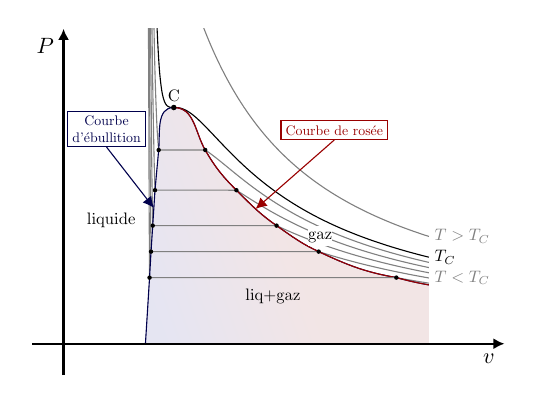
\begin{tikzpicture}
	\message{PV diagram - Maxwell construction^^J}
	\def\xmax{4}
	\def\ymax{4}
	\def\N{110}
	\def\s{0.6}
	\def\A{3}
	\def\isotherm#1#2{{ \A*(8*#2)/(3*#1-1) - 3*\A/(#1*#1) }}
	% reduced equation of state
	\coordinate (C) at (\s,\A);

	% LINE
	\foreach \i/\T/\pe in {0/.75/.28,1/.8/.39,2/.85/.5,3/.9/.65,4/.95/.82,5/1.0/1,6/1.2/1}{
			\begin{scope}
				\clip (-0.15*\xmax,0) rectangle (1.15*\xmax,\ymax);
				\ifthenelse{\i = 5}{
				\draw[black,variable=\x,
				domain=0.36:{.96*\xmax/\s},
				range=0:1,samples=\N,smooth,name path=isotherm]
				plot (\s*\x,\isotherm{\x}{\T})
				node[black,right,scale=0.6] {$T_C$};
				}{
				\ifthenelse{\i = 1}{
				\draw[gray,
				variable=\x,
				domain=0.36:{.96*\xmax/\s},
				range=0:1,samples=\N,smooth,name path=isotherm]
				plot (\s*\x,\isotherm{\x}{\T})
				node[gray,right,scale=0.6] {$T < T_C$};
				}{
				\ifthenelse{\i = 6}{
				\draw[gray,
				variable=\x,
				domain=0.36:{.96*\xmax/\s},
				range=0:1,samples=\N,smooth,name path=isotherm]
				plot (\s*\x,\isotherm{\x}{\T})
				node[gray,right,scale=0.6] {$T > T_C$};
				}{
				\draw[gray,
				variable=\x,
				domain=0.36:{.96*\xmax/\s},
				range=0:1,samples=\N,smooth,name path=isotherm]
				plot (\s*\x,\isotherm{\x}{\T});
				}
				}
				}
				\ifthenelse{\i < 5}{ %\lengthtest{\pe pt < 1 pt}
					\path[name path={pe}] (0,\A*\pe) --++ ({.96*\xmax/\s},0);
					\path[name intersections={of=isotherm and pe,name=pe\i}];
				}

			\end{scope}
		}

	\begin{scope}
		\clip (0,0) rectangle (.96*\xmax,.96*\ymax);
		\fill[top color=myblue!10,bottom color=myred!10,
			middle color=myred!10,shading angle=110,
			draw=mydarkblue,thin,use Hobby shortcut]
		(.06*\xmax,0) --
		(pe0-1) --
		(pe1-1) --
		(pe2-1) --
		coordinate (E)
		(pe3-1) --
		(pe4-1)
		to[out=85,in=180]
		(C)
		to[out=0,in=120]
		(pe4-3) to[out=-60,in=135]
		(pe3-3) to[out=-45,in=145]
		(pe2-3) to[out=-35,in=155]
		(pe1-3) to[out=-25,in=170]
		(pe0-3) to[out=-15,in=170]
		(.97*\xmax,.185*\ymax) |- (0,0);
		\draw[mydarkred,thin,use Hobby shortcut]
		(C)
		to[out=0,in=120]
		(pe4-3) to[out=-60,in=135]
		(pe3-3) to[out=-45,in=145]
		coordinate (R)
		(pe2-3) to[out=-35,in=155]
		(pe1-3) to[out=-25,in=170]
		(pe0-3) to[out=-15,in=170]
		(.97*\xmax,.185*\ymax) |- (0,0);
	\end{scope}
	\node[above left=15pt and 3pt, scale=0.6] at (pe0-1) {\strut liquide};
	\node[above left=2pt and -5pt, scale=0.6, fill=white, inner sep=0] at (pe1-3) {\strut gaz};
	\node[below=1pt, scale=0.6] at ($(pe0-1)!0.5!(pe0-3)$) {\strut liq+gaz};

	% MAXWELL CONSTRUCTION
	\fill (C) circle (1pt) node[above, scale=.6] {C};
	\foreach \i in {0,1,2,3,4}{
			\draw[thin,gray] (pe\i-1) -- (pe\i-3);
			\fill[black] (pe\i-3) circle (.8pt);
			\fill[black] (pe\i-1) circle (.8pt);
		}

	\node[scale=.5, draw, mydarkred] (CR) at ([shift={(1,1)}]R)
	{Courbe de rosée};
	\draw[->, mydarkred] (CR.south) -- (R);
	\node[scale=.5, draw, mydarkblue, align=center] (CE) at ([shift={(-.6,1)}]E)
	{Courbe\\d'ébullition};
	\draw[->, mydarkblue] (CE.south) -- (E);

	% AXIS
	\draw[->,thick] (-0.2*\xmax,-0.1*\ymax) -- (-.2*\xmax,\ymax)
	node[anchor=north east,inner sep=4,scale=0.8] {$P$};
	\draw[->,thick] (-0.3*\xmax,0) -- (1.20*\xmax,0)
	node[anchor=north east,inner sep=4,scale=0.8] {$v$};

\end{tikzpicture}

\end{document}
